\chapter{Исследовательская часть}

В данной части приведены примеры работы программа, а также проведён сравнительный анализ алгоритмов при различных ситуациях на основе полученных данных.

\section{Технические характеристики}

Технические характеристики устройства, на котором выполнялось тестирование:

\begin{itemize}
	\item операционная система Windows 11 домашняя~\cite{windows11};
	\item память 16 Гбайт;
	\item процессор Intel(R) Core(TM) i5-10300H CPU с тактовой частотой 2.50ГГц.~\cite{intel_i5}
\end{itemize}


\section{Результаты исследования}

Для сравнения эффективности последовательного и параллельного алгоритмов проверки связности графа были проведены замеры времени выполнения на графах различного размера.
В качестве входных данных использовались графы с количеством вершин от 300 до 3000.
Для каждого размера графа проводилось 100 измерений, после чего в качестве итогового значения времени использовалось среднее арифметическое.

Результаты представлены на рисунке~\ref{fig:time-compare}.


\begin{figure}[H]
    \centering
    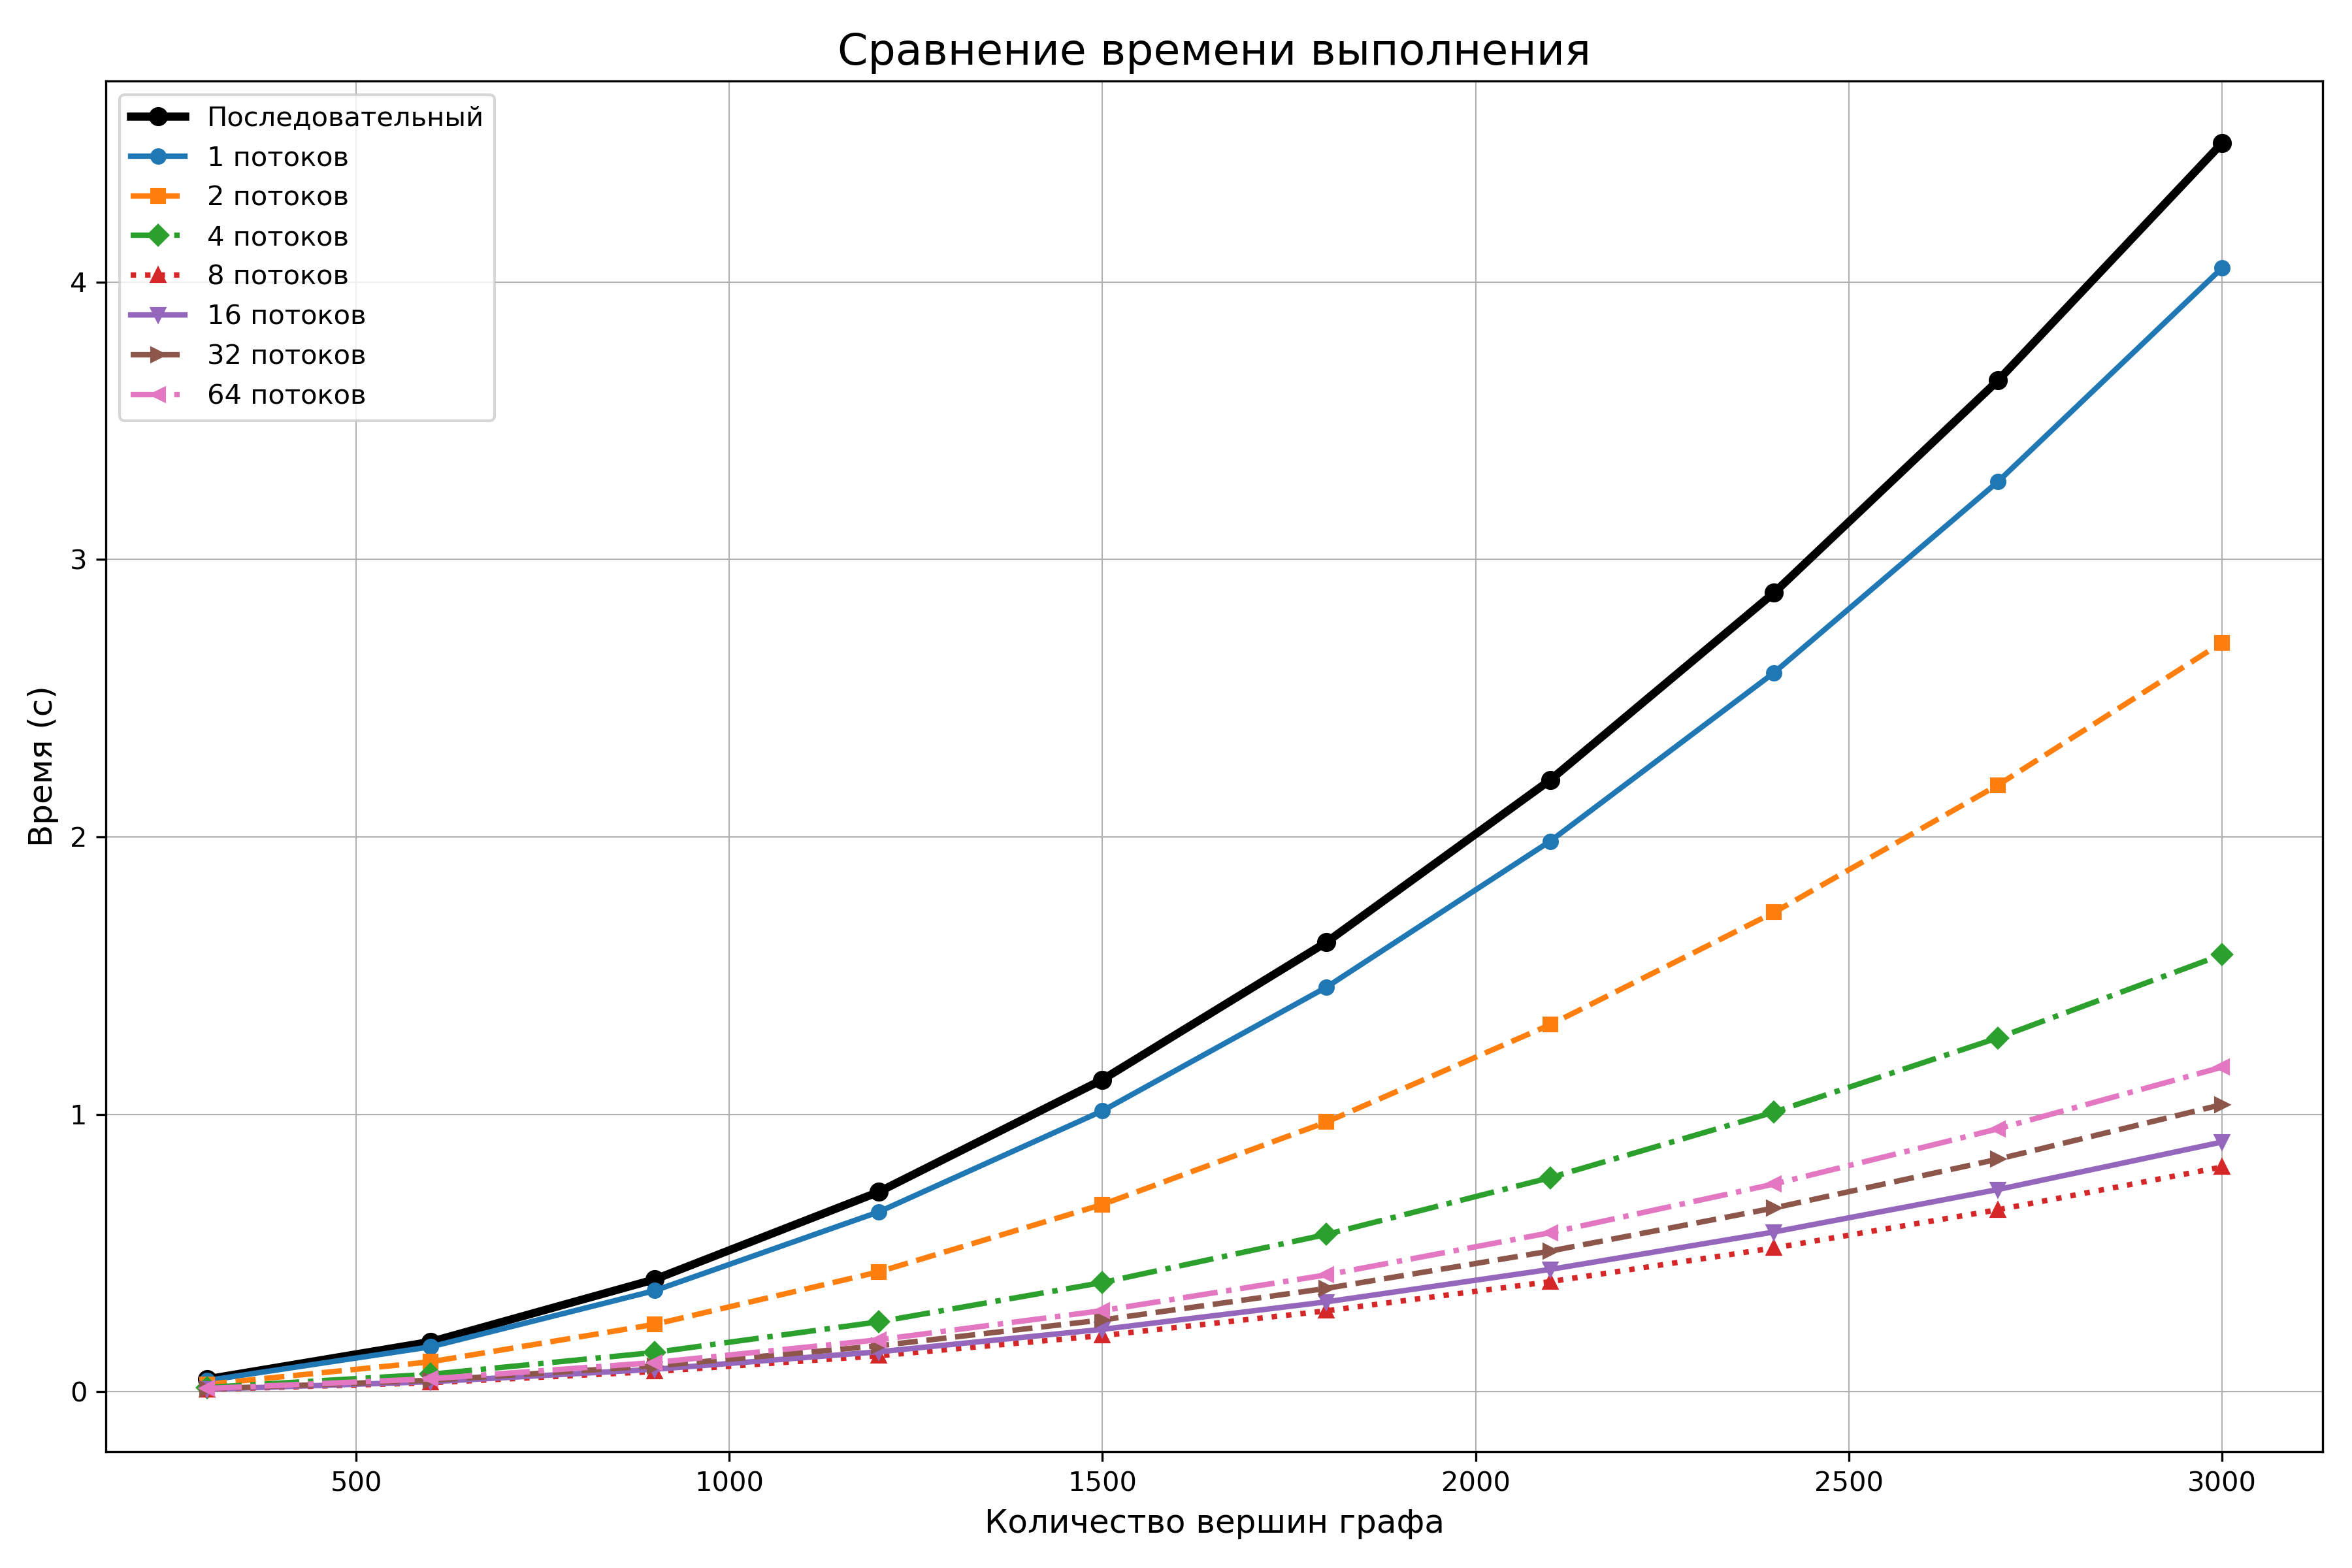
\includegraphics[width=0.95\textwidth]{images/graph_result.png}
    \caption{Сравнение времени выполнения последовательного и параллельного алгоритмов проверки связности}
    \label{fig:time-compare}
\end{figure}

\section*{Вывод}

В результате проведённого исследования было установлено, что параллельная версия алгоритма проверки связности графа показывает лучшую производительность по сравнению с последовательной версией, особенно при увеличении размера входного графа. Однако при использовании большого количества потоков наблюдается уменьшение прироста производительности из-за накладных расходов на синхронизацию и конкуренцию за общие структуры данных.

\clearpage
